\documentclass[12pt]{article}

% --- Core Math Packages ---
\usepackage{amsmath}
\usepackage{amssymb} % Provides \mathbb, \mathfrak, etc.
\usepackage{amsfonts} % Provides math fonts
\usepackage{amsthm}   % Theorem environments
\usepackage{mathtools} % Extends amsmath, e.g., \coloneqq
\usepackage{mathrsfs}  % Provides \mathscr
\usepackage{tikz-cd} % For commutative diagrams

% --- Page Layout & Typography ---
\usepackage{geometry} % For margin control
\usepackage{lmodern} % Use Latin Modern fonts (pairs well with T1)
\usepackage[T1]{fontenc} % Font encoding (improves copy-paste, hyphenation)
\usepackage[utf8]{inputenc} % Input encoding (allows UTF-8 characters)
\usepackage{microtype} % Improved typography (subtle adjustments)
\usepackage[english]{babel} % For hyphenation etc.

% --- Graphics, Links, Lists, Tables ---
\usepackage{graphicx} % For including images
\usepackage{hyperref} % For clickable links (references, URLs)
\usepackage{tikz}     % For drawing diagrams
\usepackage{enumitem} % For customizing lists
\usepackage{booktabs} % For professional-looking tables
\usepackage{url}      % For typesetting URLs

% --- Page Geometry ---
\geometry{margin=1in} % Set 1-inch margins on all sides

% --- Theorem Environments ---
\newtheorem{definition}{Definition}[section]
\newtheorem{lemma}{Lemma}[section]
\newtheorem{proposition}{Proposition}[section]
\newtheorem{corollary}{Corollary}[section]
\newtheorem{theorem}{Theorem}[section]

% --- Custom Math Commands ---
\DeclareMathOperator{\arsinh}{arsinh}

% --- Document Metadata ---
\title{Arithmetic Expression Geometry I: Flow, Torsion, and the First Kind Expression Space}
\author{Mingli Yuan \\
        \texttt{mingli.yuan@gmail.com}}
\date{\today}

% --- Hyperref Setup ---
\hypersetup{
    colorlinks=true,
    linkcolor=blue,
    filecolor=magenta,
    urlcolor=cyan,
    citecolor=green,
    pdftitle={\@title},
    pdfauthor={\@author},
    pdfkeywords={Arithmetic Expressions, Hyperbolic Geometry, Flow Equation, Geometric Group Theory, Computational Geometry, Arithmetic Torsion},
    bookmarks=true,
    bookmarksopen=true,
}

% --- Document Start ---
\begin{document}

\maketitle

\begin{abstract}
We introduce a novel geometric framework, \emph{Arithmetic Expression Geometry} (AEG), which interprets arithmetic expressions as propagating structures embedded in curved geometric spaces. This paper constructs the foundational model---the \emph{first kind expression space} \( \mathfrak{E}_1 \)---on the upper half-plane with a hyperbolic metric structure. We derive a flow equation governing the propagation of values along arithmetic paths and show that the assignment function \( a = -x/y \) satisfies this flow equation. For the standard Poincaré metric case (\(\mu=1, \lambda=1\)), \(a\) is also an eigenfunction of the Laplacian with eigenvalue -2. We establish a precise correspondence between local arithmetic torsion, which captures the non-commutativity of addition and multiplication, and hyperbolic area in grid structures embedded in \( \mathfrak{E}_1 \). Furthermore, we define a global arithmetic torsion for arbitrary expression paths and prove a triple identity relating it to a geometric area integral within a specially constructed 'accumulative commutative space', providing a Stokes-like theorem for arithmetic. Finally, we introduce the tube structure \( \mathcal{T} \) to study parameterized expression families. This work establishes the theoretical foundation for a geometry of computation rooted in arithmetic structure.
\end{abstract}

\tableofcontents
\newpage

\section{Introduction}

\subsection{Historical Context and Motivation}
The study of arithmetic expressions has deep roots, extending from foundational work on formal grammars and rewriting systems (e.g., Post\cite{Post1943FormalRO}, Chomsky\cite{Chomsky1956ThreeMF}) to the development of type theory and lambda calculus aimed at taming paradoxes and managing computational semantics (e.g., Church\cite{Church1940AFO}, Martin-L\"{o}f\cite{MartinLf1975AnIT}). These traditions primarily treat expressions as symbolic or algebraic objects—trees, terms, strings—subject to syntactic rules and evaluation procedures. While powerful, this perspective often overlooks potential intrinsic geometric structures. This leads to a fundamental question, largely unexplored: \textit{Can the very process of arithmetic evaluation manifest as a geometric phenomenon?} Can expressions trace paths, define flows, and inhabit spaces shaped by the operations themselves?

\subsection{Main Research Question}
This paper addresses the central theoretical question:
\begin{center}
\emph{Can the dynamics of evaluating arithmetic expressions be intrinsically encoded in a geometric space, with propagation governed by inherent rules?}
\end{center}
We propose such a geometry exists, where fundamental operations like addition and multiplication correspond to motions along distinct directions within a curved space, and the evaluation process unfolds dynamically as a geometric flow. In this view, arithmetic operations generate not just numbers, but geometric structures: they induce \emph{flows}, accumulate \emph{torsion}, and define \emph{paths} through dedicated mathematical spaces.

\subsection{Core Contributions}
This paper, the first in a planned series, establishes the foundations of Arithmetic Expression Geometry by presenting its major contributions:
\begin{enumerate}[label=\textbf{C\arabic*.}, leftmargin=*, widest=C5, align=left]
  \item We define \textbf{threadlike arithmetic expressions} and formalize their representation via curried path notation, providing a tractable model for sequential computation.
  \item We derive the \textbf{arithmetic flow equation} that governs how expression values propagate along these paths and demonstrate its interpretation as a special Eikonal equation from geometric optics and mechanics.
  \item We construct the \textbf{first kind arithmetic expression space} \( \mathfrak{E}_1 \) on the upper half-plane equipped with a general hyperbolic metric structure, where the assignment function \( a = -x/y \) satisfies the flow equation and is a Laplacian eigenfunction.
  \item We introduce \textbf{arithmetic torsion}, quantifying the non-commutativity of addition and multiplication, and establish both a local correspondence to hyperbolic area in \( \mathfrak{E}_1 \) and a global integral identity in a separate 'accumulative commutative space'.
  \item We propose the \textbf{tube structure} \( \mathcal{T} \), formed by parameterizing families of expression spaces, providing a framework to study the dynamics of expressions and the evolution of their zero loci across parameters.
\end{enumerate}

\subsection{Organization of the Paper}
The remainder of this paper is structured as follows:
\begin{itemize}
  \item \textbf{Section 2} formally defines arithmetic expressions as paths using production rules, currying, and path notation, focusing on threadlike and alternating structures.
  \item \textbf{Section 3} derives the arithmetic flow equation from infinitesimal generation principles and analyzes its Eikonal, Hamilton-Jacobi, and contour-gradient forms.
  \item \textbf{Section 4} constructs the first kind space \( \mathfrak{E}_1 \), establishes its metric structure, and proves the properties of the assignment function \(a=-x/y\).
  \item \textbf{Section 5} investigates geometric phenomena within \( \mathfrak{E}_1 \), including expression propagation mechanisms, dual grid structures related to Baumslag–Solitar groups, and the local torsion-area correspondence.
  \item \textbf{Section 6} introduces global arithmetic torsion, the accumulative commutative space, and establishes an integral theorem for torsion.
  \item \textbf{Section 7} introduces the tube structure \( \mathcal{T} \) as a family of \( \mathfrak{E}_1 \) spaces, discussing sections, trajectories, and the potential for complex zero locus evolution.
  \item \textbf{Section 8} provides a discussion of the results and outlines future research directions, including curvature interpretations, integral theorems, and connections to other mathematical fields.
\end{itemize}

\section{Threadlike Expressions and Arithmetic Paths}

\subsection{Arithmetic expression}\label{subsec:arithmetic-expression-full}
In order to define arithmetic expressions involving real numbers  $\mathbb{R}$ in a rigorous way, we need to use a sophisticated type theory.
However, in order to keep things simple and maintain clarity, we will start by using only production rules, but with certain semantic restrictions.
We will also begin with rational numbers $\mathbb{Q}$ to avoid the difficulties inside real numbers $\mathbb{R}$ .

\begin{definition}\label{def:arithmetic-expression-full}
    An arithmetic expression $a$ over $\mathbb{Q}$ is a structure given by the following production rules:
\begin{equation}\label{eq:productionrule-full}
\begin{aligned}
a &\longleftarrow x\\
a &\longleftarrow ( a + a )\\
a &\longleftarrow ( a - a )\\
a &\longleftarrow ( a \times a )\\
a &\longleftarrow ( a \div a )
\end{aligned}
\end{equation}
    where $x \in \mathbb{Q}$, and we denote this as $a \in \mathbb{E} \left [\mathbb{Q} \right ]$.
\end{definition}

During the production process, we can obtain both a string representation and a tree representation of arithmetic expression $a$,
where the two representations are equivalent.
For instance, the string representation of $a$ might be:
\begin{equation}
(((((1 \times 2) \times 2) - 1) \times (2 + 1)) - 6)\label{eq:equation-full}
\end{equation}
and the parsed syntax tree is depicted in Figure~\ref{fig:syntaxtree-full}.

\begin{figure}[ht]
\centering
\resizebox{0.2\textheight}{!}{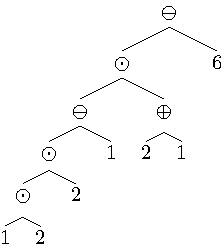
\includegraphics{images/02-example-expression-syntax-tree.pdf}}
\caption{a tree representation of an arithmetic expression}\label{fig:syntaxtree-full}
\end{figure}

Evaluation $\nu$ is a partial function that operates on arithmetic expression $a \in \mathbb{E} \left [\mathbb{Q} \right ]$.
It is undefined only if division by zero occurs during the recursive evaluation process.
We can define evaluation $\nu(a)$ of $a$ recursively as follows:
\begin{itemize}
  \item Constant leaf: for any $x \in \mathbb{Q}$, $\nu(x) = x$.
  \item Compositional node by $+$: For any $(a + b)$, $\nu((a + b)) = \nu(a) + \nu(b)$.
  \item Compositional node by $-$: For any $(a - b)$, $\nu((a - b)) = \nu(a) - \nu(b)$.
  \item Compositional node by $\times$: For any $(a \times b)$, $\nu((a \times b)) = \nu(a) \nu(b)$.
  \item Compositional node by $\div$: For any $(a \div b)$, if $\nu(b) \neq 0$, then $\nu((a \div b)) = \nu(a) / \nu(b)$.
\end{itemize}

We say that an arithmetic expression $a$ is \emph{evaluable} if $\nu(a)$ is defined.
In the rest of this article, we will only consider evaluable arithmetic expressions unless stated otherwise.

\begin{definition}
The evaluation order of an arithmetic expression $a$ is an ordering of branch nodes in the tree representation of $a$
such that every node (sub-expression) is evaluated before its parent.
\end{definition}

\begin{definition}
A threadlike expression is an arithmetic expression that all the left nodes in its tree representation are leaf nodes.
\end{definition}
So a threadlike expression is right-expanded and its evaluation order is unique.
Threadlike expressions are significant here because they are analogous to the concept of paths in homotopy theory in geometry.

\subsection{Currying and path notation}\label{subsec:currying-full}
Currying is a basic technique in functional programming\cite{Reynolds1972DefinitionalIF},
which is used to transform a function with multiple arguments into a sequence of functions with one argument.
By currying a threadlike arithmetic expression, we can obtain a sequence of functions that operate on an operand, which is the leftmost leaf node.

We introduce the following notation for currying a threadlike arithmetic expression:
\begin{itemize}
    \item initial operand: the leftmost leaf node
    \item operator: $\oplus_y: x \mapsto x + y$
    \item operator: $\ominus_y: x \mapsto x - y$
    \item operator: $\otimes_y: x \mapsto x \cdot e^y$
    \item operator: $\oslash_y: x \mapsto x \cdot e^{-y}$
\end{itemize}

Suppose we have a series of operators $a_1, a_2, \cdots a_{n-1}, a_n$, we introduce a \emph{path notation}.
\[x a_1 a_2 \cdots a_{n-1} a_n \coloneqq a\_n( a_{n-1}( \cdots a_2( a_1(x) ) \cdots ) )\]
If a path begins with a number, we refer to it as a \emph{bounded path}.
If it does not, we refer to it as a \emph{free path}.

\begin{lemma}\label{lemma:associative-full}
    The operators within a path are associative.
\end{lemma}
\begin{proof}
This follows directly from the associativity of function composition. For free paths represented by functions $\mathbf{a}, \mathbf{b}, \mathbf{c}$, we have $\mathbf{c} \circ (\mathbf{b} \circ \mathbf{a}) = (\mathbf{c} \circ \mathbf{b}) \circ \mathbf{a}$.
\end{proof}

\begin{definition}\label{definition:concatenate-full}
    The concatenation of paths $p_1 \cdot p_2$ is defined as the composite of functions:
    \[p_1 \cdot p_2 \coloneqq p_2 \circ p_1 \]
\end{definition}

\subsection{Alternating threadlike expressions}\label{subsec:alternating-full}
Now we can define alternating threadlike expressions using the path notion.
\begin{equation}\label{eq:alternative-full}
    \alpha = a_1 b_1 a_2 b_2 \cdots a_l b_l, a_i = \otimes_{\lambda_i}, b_i = \oplus_{\mu_i}, \lambda_i, \mu_i \in \mathbb{R}
\end{equation}
Any arithmetic expression can be converted into an alternating threadlike expression by introducing identity elements ($0$ for addition, $1$ for multiplication). So it is a kind of canonical form. We can derive a formula for perturbations in such expressions. Let $\hat{\lambda}_i$ be the right-accumulated sum of $\lambda_j$. For a starting point $\mu_0$ and its perturbation $\tilde{\mu}_0$, we have:
\begin{equation}
\frac{\alpha(\tilde{\mu}_0) - \alpha(\mu_0)}{\tilde{\mu}_0 - \mu_0} = e^{\hat{\lambda}_l} = e^{\sum_{j=1}^l \lambda_j}\label{eq:ratio-full}
\end{equation}
This shows the perturbation along the path is controlled by the multiplication terms.

\subsection{Generated structure, commutator and arithmetic torsion}\label{subsec:generated-structure-full}
We consider the algebraic structure freely generated by the path operators. This forms a group, but it is not abelian. The commutator of the generators is generally not identity:
\begin{equation}
x \oplus_\mu \otimes_\lambda \ominus_\mu \oslash_\lambda - x = \mu(1 - e^{-\lambda})\label{eq:commutator1-full}
\end{equation}
Or equivalently, we define the difference $\tau$ which we call \textbf{arithmetic torsion}:
\begin{equation}
\tau = x \oplus_\mu \otimes_\lambda - x \otimes_\lambda \oplus_\mu = \mu(e^\lambda - 1)\label{eq:torsion-full}
\end{equation}
This constant difference indicates a type of torsion in the generated group.

\subsection{Levels of Equality, Singularity, and Symmetry Problems}
\label{subsec:problems-on-equality-singularity-symmetries-full}
It is useful to consider different levels of equality:
\begin{enumerate}
    \item \textbf{Literal Equality}: Identical sequences of operations.
    \item \textbf{Operational/Syntactic Equality}: Equality under rules like associativity.
    \item \textbf{Relational/Algebraic Equality}: Equality under additional imposed relations.
    \item \textbf{Semantic Equality}: Equality of the final numerical evaluation.
\end{enumerate}
Significant theoretical challenges arise from the "distance" between these levels, leading to foundational problems:
\begin{itemize}
    \item \textbf{Singularity Problem}: Syntactically valid expressions may be semantically invalid (e.g., division by zero). How do these manifest in the geometric model?
    \item \textbf{Symmetry Problem}: What is the relationship between the symmetries of the algebraic structure and the symmetries of the final geometric space?
\end{itemize}
Exploring these problems is central to our research.

\section{The Arithmetic Flow Equation}

This section derives the central flow equation governing how assignment values propagate through geometric space: $\frac{da}{ds} = \mu \cos \theta + a \lambda \sin \theta$, where $\theta$ represents the angle of movement. The flow equation can be reformulated in various ways, including its coordinate-free form ($||\nabla a|| = \sqrt{\mu^2 + a^2 \lambda^2}$), which is an Eikonal equation equivalent to a special Hamilton-Jacobi equation.

The section demonstrates that the flow equation is consistent with discrete generating processes and can be expressed in contour-gradient form. It establishes a relationship between arithmetic torsion and geometric area ($d\tau = \mu \lambda du dv$), linking non-commutativity in arithmetic to measurable geometric properties. The flow equation is shown to have a geometric propagation interpretation, where assignment values correspond to wavefront evolution in hyperbolic space. The section concludes with a discussion of the existence of metrics that make functions satisfy the flow equation, presenting a local morphing process while noting that the global case remains unsettled.

\subsection{Derivation of the flow equation}\label{sec:equation-full}

Consider an infinitesimal generating process on a Riemannian surface $M$ using two generators:
one for an additional action $\mu$ and the other for a multiplicative action $e^\lambda$.
These two generators are perpendicular.
This generation process produces an assignment $A: M \to R$ over the surface.

For any point with an assignment $a_0$, if we consider a movement of distance $\epsilon$ in a direction with angle $\theta$
over a time period of $\delta$, we can establish the following:

\[
    a_{\delta} = (a_0 + \mu \epsilon \cos \theta)e^{\lambda \epsilon \sin \theta}
\]

or

\[
    a_{\delta} = a_0 e^{\lambda \epsilon \sin \theta} + \mu \epsilon \cos \theta
\]

Both formula can be simplified to the same result:

\[
    a_{\delta} = a_0 + \epsilon (a_0 \lambda \sin \theta + \mu \cos \theta)
\]

Then, we have the following equation:

\[
    \frac{1}{\delta} (a_{\delta} - a_0) = \frac{\epsilon}{\delta} (\mu \cos \theta + x_0 \lambda \sin \theta)
\]

When both $\delta$ and $\epsilon$ are towards zero, we get $da / dt$, and hence

\[
    \frac{da}{dt} = u (\mu \cos \theta + a \lambda \sin \theta)
\]

Or, we can change it to another form

\begin{equation}
    \frac{da}{ds} = \mu \cos \theta + a \lambda \sin \theta\label{eq:flow-full}
\end{equation}

We name this equation~\eqref{eq:flow-full} as the flow equation.

The left side of this equation is governed by the distance structure, while the right side is governed by the angle structure.
So that the isometrics of the surface keep the flow equation~\eqref{eq:flow-full}.

We can also get a direct formal solution of the flow equation~\eqref{eq:flow-full}(details in Appendix~\ref{sec:directformalsolution}).

\begin{equation}
   a = (a_0 + \frac{\mu}{\lambda} \cot \theta) e^{\lambda s \sin \theta} - \frac{\mu}{\lambda} \cot \theta\label{eq:solution-full}
\end{equation}

\subsection{The contour-gradient form of flow equation}\label{subsec:the-contour-gradient-form-full}

It is easy to derive the contour equation in the local coordinate

\begin{equation}
    \mu \cos \theta_c + a \lambda \sin \theta_c = 0\label{eq:contour-full}
\end{equation}

then we have

\begin{equation}
    \theta_c = - \arctan \frac{\mu}{a \lambda}\label{eq:contourangle-full}
\end{equation}

the contour and the gradient are perpendicular to each other

\begin{equation}
    \theta_g = \pm \frac{\pi}{2} - \arctan \frac{\mu}{a \lambda}\label{eq:gradientangle-full}
\end{equation}

then along $\theta_g$ we have

\begin{equation}
    \frac{da}{ds} = \mu \cos (\pm \frac{\pi}{2} - \arctan \frac{\mu}{a \lambda}) + a \lambda \sin (\pm \frac{\pi}{2} - \arctan \frac{\mu}{a \lambda})
    \label{eq:alonggradient-full}
\end{equation}

\begin{equation}
    \frac{da}{ds} = \pm \sqrt{\mu^2 + \lambda^2 a^2}\label{eq:grad-full}
\end{equation}

By introducing the right-hand rotation angle $\phi$ along the gradient direction, we can establish a local polar coordinate system based on the gradient and contour lines.
Then the growth rate of $a$ along the angle $\phi$ is

\begin{equation}
    \frac{da}{ds} = \sqrt {\mu^2 + a^2 \lambda^2} \cos \phi\label{eq:contourgradient-full}
\end{equation}

\subsection{Arithmetic coordinate and area formula}\label{subsec:descartes-coordinate-full}
We begin our exploration by examining the flow equation~\eqref{eq:flow-full} within the framework of a local polar coordinate system:
\begin{equation}
    \frac{da}{ds} = \mu \cos \theta + a \lambda \sin \theta
\end{equation}
In an effort to re-contextualize this equation, we set $du = \cos \theta ds$ and $dv = \sin \theta ds$,
where $du$ and $dv$ are perpendicular infinitesimal movements.
This enables us to express the flow equation in a different light:
\begin{equation}
    da = \mu du + a \lambda dv
\end{equation}
Our attention now turns to the concept of arithmetic torsion, particularly at an infinitesimal level.
Delving into the interplay between two infinitesimal generating processes, we observe that:
\begin{equation}
    d\tau = (a_0 + \mu du) e^{\lambda dv} - (a_0 e^{\lambda dv} + \mu du)
\end{equation}
From this relationship, we deduce:
\begin{equation}
    d\tau = \mu du (e^{\lambda dv} - 1)
\end{equation}
This leads us to an area formula, capturing the essence of this interaction:
\begin{equation}
    d\tau = \mu \lambda du dv \label{eq:area_formula-full}
\end{equation}

\subsection{The coordinate-free form of flow equation}\label{subsec:coordinate-free-full}
From the contour-gradient form of the flow equation, we can derive a coordinate-free form of the flow equation.
Let's consider the direction of \(\phi = 0\) in the contour-gradient coordinate system, and we have
\[
    \frac{da}{ds}|_{\phi = 0} = \sqrt{\mu^2 + a^2 \lambda^2} \cos 0
\]
Notice the gradient of \(a\) is not dependent on the coordinate system, and we have the coordinate-free form of the flow equation:
\begin{equation}\label{eq:coordinate-free-full}
||\nabla a|| = \sqrt{\mu^2 + a^2 \lambda^2}
\end{equation}
It should be noted that the coordinate-free form of the flow equation is an Eikonal equation,
and can be viewed as a special Hamilton–Jacobi equation
\[
H(x, a, \nabla a) = 0
\]
where the Hamiltonian is
\begin{equation}\label{eq:hamiltonian-full}
    H(x, a, p) = ||p|| - \sqrt{\mu^2 + a^2 \lambda^2}
\end{equation}

\section{The First Kind Expression Space $\mathfrak{E}_1$}

This section introduces the first kind arithmetic expression space ($\mathfrak{E}_1$), providing a geometric framework for analyzing arithmetic expressions. The space is constructed on the upper half-plane with a hyperbolic metric: $ds^2 = \frac{1}{y^2} (dx^2 + dy^2)$, where the assignment function $a = - \frac{x}{y}$ satisfies the flow equation and serves as an eigenfunction of the Laplacian with eigenvalue 2.

Two equivalent examples of $\mathfrak{E}_1$ are presented: the upper half-plane model and a horocycle-based coordinate system, connected through Möbius transformation. The section explores geometric propagation mechanisms, showing how the assignment value propagates like expanding concentric circles in hyperbolic space. It examines grid structures in $\mathfrak{E}_1$, revealing dual grids reflecting the geometric structure of the Baumslag-Solitar group, and demonstrates how arithmetic torsion corresponds precisely to hyperbolic areas enclosed between evaluation paths. The section concludes by introducing tube structures, which extend $\mathfrak{E}_1$ to parameterized families, enabling analysis of how expressions evolve across parameter variations.

\subsection{Foundational exemplars}\label{subsec:motivexamples-full}

We present two analytically equivalent examples that belong to the class of spaces designated as the first kind arithmetic expression space $\mathfrak{E}_1$.

\subsubsection{Example 1: Upper Half Plane Model}

Consider the upper half plane ${\mathcal{H}: (x, y) \ | \ y > 0}$ equipped with the following inner product and metric tensor:

$$
\mathbf{a} \cdot \mathbf{b} = \begin{bmatrix} a_x & a_y \end{bmatrix} \begin{bmatrix} \frac{1}{y^2} & 0 \\ 0 & \frac{1}{y^2} \end{bmatrix} \begin{bmatrix} b_x \\ b_y \end{bmatrix}
$$

$$
ds^2 = \frac{1}{y^2} (dx^2 + dy^2)
$$

On this manifold, we define an assignment field $a$ as follows:

\begin{equation}\label{eq:exmp1-full}
a = - \frac{x}{y}
\end{equation}

\begin{theorem}\label{thm:exmp1-full}
The assignment $a$ defined by formula \eqref{eq:exmp1-full} satisfies the flow equation \eqref{eq:flow-full}.
\end{theorem}

\begin{proof}
We initiate with the differential of the assignment:
$$
da = d\left(-\frac{x}{y}\right) = \frac{xdy - ydx}{y^2} = -\frac{dx + ady}{y}
$$

The differential of arc length is given by:
$$
ds = \frac{\sqrt{dx^2 + dy^2}}{y}
$$

Therefore:
$$
\frac{da}{ds} = - \frac{dx + ady}{y} \cdot \frac{y}{\sqrt{dx^2 + dy^2}} = - \frac{dx + ady}{\sqrt{dx^2 + dy^2}}
$$

In the local coordinate system determined by $(-1, 0)$ and $(0, -1)$ under the right-hand rule, we have:
$$
\cos \theta = \frac{-dx}{\sqrt{dx^2 + dy^2}} \quad \text{and} \quad \sin \theta = \frac{-dy}{\sqrt{dx^2 + dy^2}}
$$

Substituting these values:
$$
\frac{da}{ds} = \cos \theta + a \sin \theta
$$

This precisely corresponds to the flow equation \eqref{eq:flow-full} with $\mu=1$ and $\lambda=1$.
\end{proof}

We can verify that $a$ constitutes an eigenfunction of the Laplacian operator:
$$
\Delta a = - y^2 \left(\frac{\partial^2 a}{\partial x^2} + \frac{\partial^2 a}{\partial y^2}\right) = y^2 \left(\frac{\partial}{\partial y} \left(\frac{\partial}{\partial y} \frac{x}{y}\right)\right) = 2a
$$

\subsubsection{Example 2: Horocycle-Based Coordinate System}

For our second exemplar, we introduce a horocycle-based coordinate system for hyperbolic surfaces. This global coordinate system comprises two orthogonal families of curves: horocycles sharing the same ideal point, and geodesics perpendicular to these horocycles.

\begin{figure}[ht]
\centering
\resizebox{0.5\textwidth}{!}{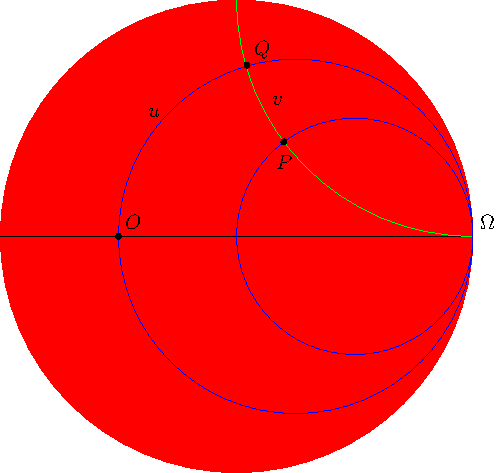
\includegraphics{images/11-horocyclebased.pdf}}
\caption{A horocycle-based coordinate system on the Poincaré disc. Blue curves represent horocycles tangent at ideal point $\Omega$, green lines depict perpendicular geodesics.}\label{fig:horocyclecoord-full}
\end{figure}

On the Poincaré disc $\mathcal{P}$, the coordinates of a point $P$ are denoted by $(u,v)$, where:
\begin{itemize}
\item $u$ represents the signed length of $OQ$
\item $v$ represents the signed length of $QP$
\item The sign conventions adhere to the right-hand rule and orientation relative to the ideal point $\Omega$
\end{itemize}

We equip this coordinate system with the inner product:
$$
\mathbf{a} \cdot \mathbf{b} = \begin{bmatrix} a_u & a_v \end{bmatrix} \begin{bmatrix} e^{-2v} & 0 \\ 0 & 1 \end{bmatrix} \begin{bmatrix} b_u \\ b_v \end{bmatrix}
$$

And the corresponding metric tensor:
$$
ds^2 = e^{-2v} du^2 + dv^2
$$

The Laplacian operator in this coordinate system is expressed as:
$$
\Delta = e^{2v} \frac{\partial^2}{{\partial u}^2} + \frac{\partial^2}{{\partial v}^2} - \frac{\partial}{\partial v}
$$

In this coordinate framework, we define an assignment:

\begin{equation}\label{eq:exmp2-full}
a = u e^{-v}
\end{equation}

\begin{theorem}\label{thm:exmp2-full}
The assignment $a$ defined by formula \eqref{eq:exmp2-full} satisfies the flow equation \eqref{eq:flow-full}.
\end{theorem}

\begin{proof}
We establish this result by demonstrating that examples 1 and 2 are equivalent through a Möbius transformation. Consider the complex representation of the upper half plane:
$$
z = x + yi
$$

The Möbius transformation mapping the upper half plane to the Poincaré disc is given by:
$$
z \mapsto \frac{z-i}{z+i}
$$

\begin{figure}[ht]
\centering
\resizebox{0.8\textwidth}{!}{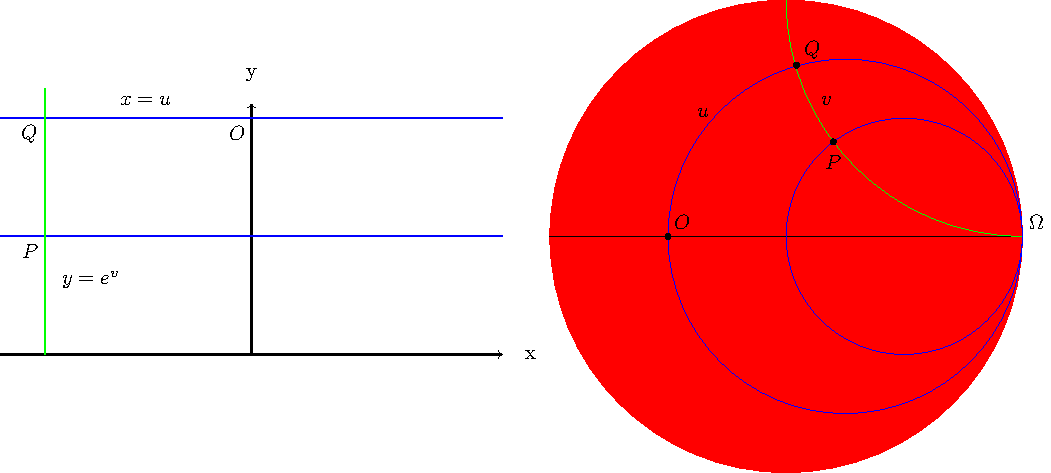
\includegraphics{images/12-proofbymapping.pdf}}
\caption{Mapping between the upper half plane and Poincaré disc models}\label{fig:mapping-full}
\end{figure}

This conformal transformation maps horizontal lines in $\mathcal{H}$ to horocycles sharing the ideal point $\Omega = 1$ in $\mathcal{P}$, and vertical geodesics in $\mathcal{H}$ to perpendicular geodesics in $\mathcal{P}$.

Expressed in the target coordinate system, this transformation yields:
$$
\begin{cases}
x = u\\
y = e^v \\
\end{cases}
$$

Substituting into the assignment from Example 1:
$$
a = -\frac{x}{y} = -\frac{u}{e^v} = -u e^{-v}
$$

Since the Möbius transformation is conformal and preserves the flow equation, and accounting for the orientation change, we obtain $a = u e^{-v}$ satisfying the flow equation.
\end{proof}

As in Example 1, we can verify that $a$ constitutes an eigenfunction of the Laplacian:
$$
\Delta a = e^{2v} \frac{\partial^2(u e^{-v})}{{\partial u}^2} + \frac{\partial^2(u e^{-v})}{{\partial v}^2} - \frac{\partial(u e^{-v})}{\partial v} = 2a
$$

These two examples, emerging from the same geometric foundation but expressed in different coordinate systems, demonstrate the fundamental properties of the first kind arithmetic expression space.

\subsection{Theoretical framework of $\mathfrak{E}_1$ space}\label{subsec:generalframework-full}

Building upon the foundational exemplars, we now establish a comprehensive theoretical framework for the first kind arithmetic expression space $\mathfrak{E}_1$. 

Consider the upper half plane $\mathcal{B}$:
$$
\{\mathcal{B}: (x, y) | y > 0 \}
$$

equipped with an inner product and metric tensor parameterized by constants $\mu$ and $\lambda$:

$$
\mathbf{a} \cdot \mathbf{b} = \begin{bmatrix} a_x & a_y \end{bmatrix} \begin{bmatrix} \frac{1}{\mu^2 y^2} & 0 \\ 0 & \frac{1}{\lambda^2 y^2} \end{bmatrix} \begin{bmatrix} b_x \\ b_y \end{bmatrix}
$$

$$
ds^2 = \frac{1}{y^2}\left(\frac{dx^2}{\mu^2} + \frac{dy^2}{\lambda^2}\right)
$$

The assignment function in this generalized framework maintains the form:

\begin{equation}\label{eq:genassignment-full}
a = - \frac{x}{y}
\end{equation}

This defines the first kind arithmetic expression space $\mathfrak{E}_1$, characterized by the following theorem:

\begin{theorem}\label{thm:generalE1-full}
The assignment $a$ given by \eqref{eq:genassignment-full} satisfies the flow equation \eqref{eq:flow-full} with parameters $\mu$ and $\lambda$, independent of the specific values of these generators.
\end{theorem}

\begin{proof}
The differential of the assignment is given by:
$$
da = d\left(-\frac{x}{y}\right) = \frac{xdy - ydx}{y^2} = -\frac{dx + a dy}{y}
$$

The differential of arc length is expressed as:
$$
ds = \frac{1}{y}\sqrt{\frac{dx^2}{\mu^2} + \frac{dy^2}{\lambda^2}}
$$

Therefore:
$$
\frac{da}{ds} = - \frac{dx + a dy}{y} \cdot \frac{y}{\sqrt{\frac{dx^2}{\mu^2} + \frac{dy^2}{\lambda^2}}} = -\frac{dx + a dy}{\sqrt{\frac{dx^2}{\mu^2} + \frac{dy^2}{\lambda^2}}}
$$

In the local coordinate system determined by $(-1, 0)$ and $(0, -1)$ according to the right-hand rule:

$$
\cos \theta = \frac{-\frac{dx}{\mu}}{\sqrt{\frac{dx^2}{\mu^2} + \frac{dy^2}{\lambda^2}}} \quad \text{and} \quad \sin \theta = \frac{-\frac{dy}{\lambda}}{\sqrt{\frac{dx^2}{\mu^2} + \frac{dy^2}{\lambda^2}}}
$$

Substituting these values:
$$
\frac{da}{ds} = \mu \cos \theta + a \lambda \sin \theta
$$

This precisely corresponds to the flow equation \eqref{eq:flow-full} with the given parameters $\mu$ and $\lambda$.
\end{proof}

The $\mathfrak{E}_1$ space is distinguished by its intrinsic connection to hyperbolic geometry and the property that the assignment function $a = -x/y$ constitutes an eigenfunction of the Laplacian operator with eigenvalue 2. This space provides a natural geometric framework for analyzing arithmetic expressions, particularly those involving addition and multiplication operations.

\subsection{Tube structure}\label{sec:tubestructure-full}

In preceding sections, we introduced the first kind arithmetic expression space $\mathfrak{E}_1$ as a geometric realization of arithmetic flow under \textbf{fixed} generator parameters $\mu$ and $\lambda$. However, more complex structures emerge when we consider the entire family of spaces indexed by the parameter $\lambda$ (or potentially both $\mu$ and $\lambda$) and analyze how expression behavior evolves across this family. This naturally leads to the concept of a \emph{tube structure}.

\subsubsection{From Slices to Parameterized Families}\label{subsec:tube_slices-full}

Each individual $\mathfrak{E}_1$ space, denoted $\mathfrak{E}_1^{(\lambda)}$, can be conceptualized as a single \emph{slice} or \emph{fiber} (in the sense of fiber bundles) within the family of expression spaces indexed by the parameter $\lambda$. Within each slice, the evaluation of arithmetic expressions is realized through traversal along (geodesic) paths, the result is governed by the scalar field $a$, and the flow is determined by the metric tensor corresponding to that slice.

Consider a fixed algebraic structure—for instance, an alternating path (with a fixed internal multiplier) corresponding to a polynomial $P(x)$—and examine how its evaluation result $P(e^\lambda)$ evolves as the tube structure parameter $\lambda$ varies. For each value of $\lambda$, the evaluation $P(e^\lambda)$ corresponds to a point (or more accurately, the assignment value $a$ at that point) within the $\lambda$-slice $\mathfrak{E}_1^{(\lambda)}$. As $\lambda$ varies continuously, these points trace out a continuous trajectory through the family of spaces. We refer to such a trajectory generated by $P$ as a \emph{section} or a \emph{$\lambda$-trajectory}. The collection of all slices corresponding to the allowed $\lambda$ values, along with these structures upon them, together form a new, higher-dimensional entity: the tube structure.

\subsubsection{Tube Structure as Total Space}\label{subsec:tube_total_space-full}

We define a \textbf{tube structure $\mathcal{T}$} as the \emph{total space} formed by the family of $\mathfrak{E}_1$ spaces indexed by a continuous parameter $\lambda$ (typically $\lambda > 0$), which can be formally written as the disjoint union:
\begin{equation}
\mathcal{T} = \bigsqcup_{\lambda > 0} \mathfrak{E}_1^{(\lambda)}
\end{equation}
This total space needs to be endowed with an appropriate topology (and possibly a differential or fiber bundle structure) to support coherent analysis along the $\lambda$-direction.

In this structure:
\begin{itemize}
    \item The \emph{base space} is the parameter domain $\Lambda$ for $\lambda$ (e.g., $\mathbb{R}^+$).
    \item The \emph{fiber} over each point $\lambda$ in the base space is the geometric expression space $\mathfrak{E}_1^{(\lambda)}$.
    \item Fixed algebraic expression structures (especially those corresponding to polynomials $P(x)$, via the evaluation $P(e^\lambda)$) trace \emph{canonical sections} or $\lambda$-trajectories through $\mathcal{T}$. These sections connect the fibers for different $\lambda$.
\end{itemize}

\subsubsection{Zero Loci and Nodal Evolution}\label{subsec:tube_zeros-full}

A primary motivation for studying tube structures is to investigate how \emph{zero loci}—the sets of points where an expression evaluates to zero ($a=0$)—evolve with the parameter $\lambda$.

\begin{itemize}
    \item \textbf{In the Tube Structure $\mathcal{T}_1$ based on $\mathfrak{E}_1$}: For the $\mathfrak{E}_1$ space ($a=-x/y$) that we have discussed in detail, the zero locus within \textbf{each slice} $\mathfrak{E}_1^{(\lambda)}$ is always the \textbf{same simple} line: the y-axis ($x=0$). Consequently, in the tube structure $\mathcal{T}_1 = \bigsqcup \mathfrak{E}_1^{(\lambda)}$, the overall zero locus is the trivial hyperplane $x=0$.

    \item \textbf{Outlook for Non-Trivial Spaces}: However, as our research suggests, the simplicity of the zero locus in $\mathfrak{E}_1$ might limit its capacity to explain more complex phenomena (like those observed in knot theory examples). Therefore, there is strong motivation to seek and construct \textbf{"non-trivial" arithmetic expression spaces $\mathfrak{E}_{NT}$}, where a single slice $\mathfrak{E}_{NT}^{(\lambda)}$ might possess \textbf{multiple or morphologically more complex zero lines}. In the tube structures $\mathcal{T}_{NT}$ built from such non-trivial spaces, the zero locus itself could evolve with $\lambda$, potentially exhibiting various interesting phenomena, such as:
    \begin{itemize}
        \item \textbf{Bifurcation}: New zero lines might emerge or merge with existing ones as $\lambda$ varies.
        \item \textbf{Branching}: The zero locus of certain expressions might exhibit multi-valued behavior along the $\lambda$-direction.
        \item \textbf{Topology change}: The overall zero surface might develop handles (genus), singularities, or undergo other changes in its topological structure.
    \end{itemize}
\end{itemize}
The analysis of such complex zero loci and their evolution (potentially within $\mathcal{T}_{NT}$) constitutes a core direction for studying expression dynamics, particularly when considering families of expressions or differential equations involving $\lambda$.

\subsection{Grid structures, chirality, and their interrelation via conformal mapping}\label{subsec:grids_revised-full}

A significant geometric characteristic of the first kind arithmetic expression space ($\mathfrak{E}_1$) is the presence of two distinct yet interrelated grid structures. These structures provide a geometric realization for arithmetic operations and reveal a deep connection to the Baumslag--Solitar groups $BS(2,1)$ and $BS(1,2)$. Both grid types are constructed within the upper half-plane model $\mathcal{H} = \{(x,y) \mid y>0\}$, utilizing the assignment function $a = -x/y$ as the underlying scalar field that defines the meaning of arithmetic operations.

\subsubsection{The Rectilinear Grid: Geometric Realization of $BS(2,1)$ and its Chirality}

The first grid structure, the \textbf{rectilinear grid} (Figure~\ref{fig:grid1_revised-full}), is formed by lines parallel to the Cartesian axes.

\begin{figure}[ht]
\centering
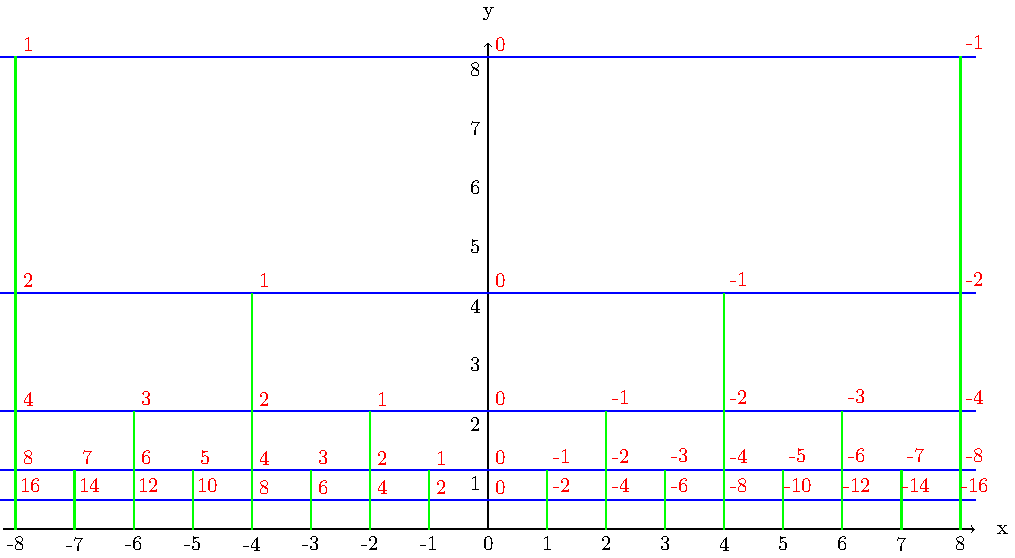
\includegraphics[width=0.8\textwidth]{images/01-grid-example-1.pdf}
\caption{Rectilinear grid structure in $\mathfrak{E}_1$, a geometric realization of $BS(2,1)$ (with multiplication factor 2), exhibiting a clockwise (right-handed) operational chirality.}\label{fig:grid1_revised-full}
\end{figure}

\subsubsection{The Transformed Grid via $w = -1/z$: Emergence of $BS(1,2)$ through Chirality Preservation}
The second grid structure, the \textbf{transformed (or curved) grid} (Figure~\ref{fig:grid2_revised-full}), results from applying the conformal transformation $w = -1/z$ to the rectilinear grid. This specific M\"obius transformation maps $\mathcal{H}$ to itself, transforming horizontal lines to semicircles and vertical lines to other semicircles. The transformed grid, under a chirality-preserving reinterpretation of its operations, serves as a geometric realization of \textbf{$BS(1,2)$}.

\begin{figure}[ht]
\centering
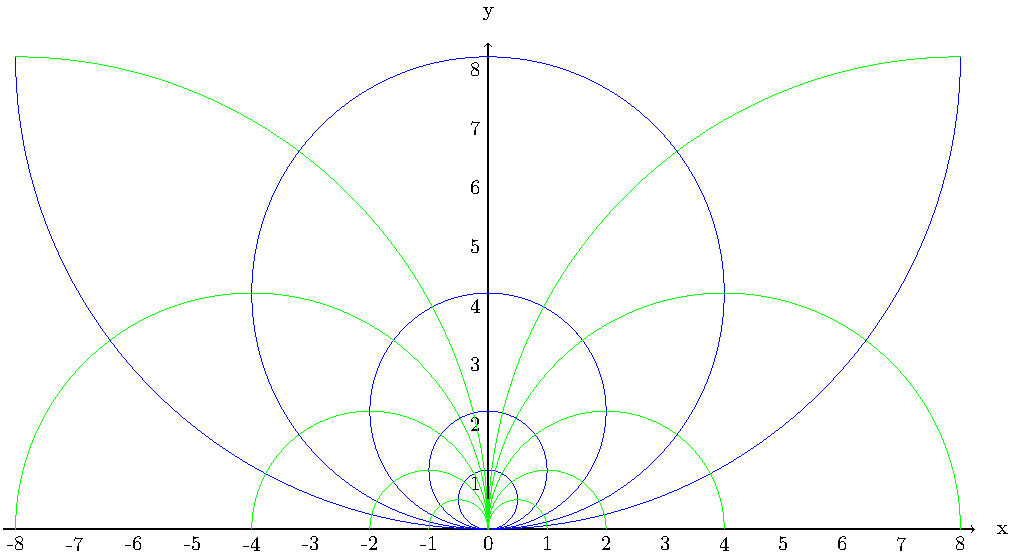
\includegraphics[width=0.8\textwidth]{images/18-grid-example-2.pdf}
\caption{Transformed (curved) grid structure in $\mathfrak{E}_1$ via $w=-1/z$. Through chirality preservation, its operations correspond to $BS(1,2)$.}\label{fig:grid2_revised-full}
\end{figure}

\section{Global Torsion and the Accumulative Commutative Space}

\subsection{Global arithmetic torsion and the accumulative commutative space}
\label{sec:global_torsion_acs_narrative_enhanced_lc}

The non-commutative nature of fundamental arithmetic operations, such as addition and multiplication, is the very source of arithmetic torsion. Consider the local effect: evaluating an expression like $x \oplus_\mu \otimes_\lambda$ versus $x \otimes_\lambda \oplus_\mu$. While both "path segments" originate from the same initial value $x$, their terminal points in the arithmetic expression space will differ if a non-zero local torsion $\tau_{\text{local}} = \nu(x \oplus_\mu \otimes_\lambda) - \nu(x \otimes_\lambda \oplus_\mu)$ exists. These two segments do not naturally form a closed loop; instead, they represent a "gap" or a "tear" caused by the order of operations. This inherent "openness" or "torn state" at the local level signifies a deviation from commutativity and poses a challenge for directly applying integral theorems like Green's or Stokes', which typically rely on closed paths or well-defined bounded regions within the space of action.

The crucial question then arises: how do these elemental "tears" accumulate along an extended, arbitrary arithmetic path $\gamma$? How can we quantify the total geometric impact of these accumulated deviations? This is the heart of the "torsion-area problem" which we previously highlighted with specific examples in the $\mathfrak{E}_1$ space and the local differential formulation $d\tau_{\text{local}} = \mu \lambda du dv$. We seek a general principle to measure this overall "deviation from commutativity" for any path $\gamma$.

Thus, the \textbf{accumulative commutative space} (ACS) is born. This space, constructed by the \textit{commutative accumulation} of operational parameters ($A_\gamma = \sum \mu_k$ and $M_\gamma = \sum \lambda_k$) from a path $\gamma$, provides exactly such a commutative canvas. Critically, in this ACS, any path $\gamma$ and its reversed-sequence counterpart $\bar{\gamma}$ share common start $(0,0)$ and end points $(A_\gamma, M_\gamma)$. This allows them to genuinely form the boundary $\partial\Sigma_\gamma$ of a well-defined planar region $\Sigma_\gamma$. It is upon this stage that we can rigorously explore and establish the geometric nature of global arithmetic torsion.

\subsubsection*{Algebraic definition of global arithmetic torsion $\tau(\gamma)$: comparison via path reversal}

Let $\gamma$ be an arbitrary arithmetic path. The \textbf{global arithmetic torsion, $\tau(\gamma)$}, is then defined through its \textbf{algebraic evaluation form}:
\begin{equation}
\tau_{\text{alg}}(\gamma) = \nu(\gamma) - \nu(\bar{\gamma})
\label{eq:T_alg_formal_final_narrative_enhanced_acs_AM_lc}
\end{equation}
A crucial property is that $\tau_{\text{alg}}(\gamma)$ is independent of the initial value $x$, making it an intrinsic characteristic of the operational structure of path $\gamma$.

\subsubsection*{Geometric representation of paths in the accumulative commutative space and the region $\Sigma_\gamma$}

The accumulative commutative space (ACS) is a Euclidean plane. For any given arithmetic path $\gamma$, its representation in this space is constructed by accumulating the parameters of its constituent operations:
\begin{itemize}
    \item $A_\gamma = \sum \mu_k$: The total accumulated additive charge.
    \item $M_\gamma = \sum \lambda_k$: The total accumulated logarithmic multiplicative charge.
\end{itemize}
When the sequence of operation parameters defining path $\gamma$ is plotted as a trajectory in this ACS, it charts a path starting from the origin $(0,0)$ to a final point $(A_\gamma, M_\gamma)$. Critically, the reversed path $\bar{\gamma}$ also maps from $(0,0)$ to the \textit{same} endpoint $(A_\gamma, M_\gamma)$, enclosing a two-dimensional region, which we denote as $\Sigma_\gamma$.

\subsubsection*{Core conclusion: the triple identity of global arithmetic torsion}

Within this framework, our central finding is that the global arithmetic torsion $\tau(\gamma)$ possesses three equivalent formulations. This \textbf{triple identity} bridges its algebraic definition with concrete geometric measures in the accumulative commutative space:

\textbf{(I) Algebraic evaluation form}:
\[ \tau(\gamma) = \nu(\gamma) - \nu(\bar{\gamma}) \]

\textbf{(II) Geometric interior integral form in the accumulative commutative space:}
\[ \tau(\gamma) = \iint_{\Sigma_\gamma} e^M dM \wedge dA \]

\textbf{(III) Geometric boundary integral form in the accumulative commutative space:}
\[ \tau(\gamma) = \oint_{\partial \Sigma_\gamma} e^M dA \]

In summary, our main theorem states the equality of these three forms:
\begin{equation}
\tau_{\text{alg}}(\gamma) = \tau_{\text{int}}(\gamma) = \tau_{\text{bound}}(\gamma)
\label{eq:triple_identity_final_narrative_enhanced_acs_AM_lc}
\end{equation}

The establishment of this triple identity provides a definitive affirmative answer to our initial "torsion-area problem": global arithmetic torsion for an arbitrary path $\gamma$ can indeed be precisely quantified as an $e^M$-weighted area within the accumulative commutative space.

\subsection{$F_2$ homomorphisms and ideal-like structures}
\label{sec:acs_algebraic_significance_revised_AM_lc}

The accumulative commutative space (ACS) also has deep algebraic significance. The set of all possible finite sequences of our fundamental operators forms the free group on two generators, $F_2 = \langle X_A, X_M \rangle$. We can define a group homomorphism $\Phi: F_2 \to \mathbb{R}^2$ by mapping any path $\gamma \in F_2$ to its total accumulated charges, $\Phi(\gamma) = (A_\gamma, M_\gamma)$.

The preimages of subgroups in $\mathbb{R}^2$ (like $k\mathbb{Z}\mu_0 \times l\mathbb{Z}\lambda_0$) form normal subgroups in $F_2$. Remarkably, the lattice structure of these normal subgroups in $F_2$ is perfectly compatible with the lattice structure of ideals in $\mathbb{Z}$ and, consequently, with the nesting of closed sets in the Zariski topology on $\text{Spec } \mathbb{Z}$. This uncovers an intrinsic arithmetic order within the purely generative framework of $F_2$, even before any notion of arithmetic evaluation $\nu(\gamma)$ is applied.

\section{Discussion and Future Directions}
This work establishes a new geometric framework for arithmetic. Key future directions include:
\begin{itemize}
    \item Formulating a general arithmetic Gauss-Bonnet theorem.
    \item Constructing non-trivial expression spaces with more complex zero loci.
    \item Deepening connections to geometric group theory, knot theory, and number theory.
\end{itemize}

\bibliographystyle{plain}
\bibliography{aeg-paper}

\end{document}

</final_file_content>

IMPORTANT: For any future changes to this file, use the final_file_content shown above as your reference. This content reflects the current state of the file, including any auto-formatting (e.g., if you used single quotes but the formatter converted them to double quotes). Always base your SEARCH/REPLACE operations on this final version to ensure accuracy.<environment_details>
# VSCode Visible Files
paper4p/aeg.tex

# VSCode Open Tabs
paper4p/aeg.tex

# Current Time
7/24/2025, 2:40:07 AM (Asia/Shanghai, UTC+8:00)

# Context Window Usage
819,180 / 1,048.576K tokens used (78%)

# Current Mode
ACT MODE
</environment_details>
